\documentclass{article}

\usepackage[english]{babel}
\usepackage[letterpaper,top=2cm,bottom=2cm,left=3cm,right=3cm,marginparwidth=1.75cm]{geometry}

\usepackage{graphicx}
\usepackage[colorlinks=true, allcolors=blue]{hyperref}
\usepackage{tabularx}
\usepackage{booktabs}
\usepackage{multirow}
\usepackage{ragged2e}
\usepackage{float}

\usepackage{algorithm}
\usepackage{algpseudocode}
\usepackage{amsmath}

\usepackage{subcaption}

\title{Generic Recommender System}
\author{
  Mateusz Bernart\\
  \texttt{156072}
  \and
  Patryk Janiak\\
  \texttt{156053}
  \and
  Marek Seget\\
  \texttt{156042}
}

\begin{document}
\maketitle

\section{Introduction}
Recommender systems are critical components for personalizing user experiences. This report details the development of a generic recommender system designed to handle diverse data sources through a unified graph-based representation. 

The primary challenge in building a generic system is the variability of dataset formats. To address this, we implement a "Convert-First" strategy. Raw data is first transformed into a standardized JSON structure, unifying user IDs, item IDs, and interaction timestamps. This unified format is then ingested by a generic interface to construct a heterogeneous graph connecting users, items, and feature nodes. This structure effectively captures complex relationships and serves as a robust foundation for training various recommendation algorithms, ranging from traditional Matrix Factorization to advanced Graph Neural Networks (GNNs).

\section{Related Work}
Recent advancements in recommender systems have increasingly leveraged graph-based methods to capture high-order connectivity between users and items. 

Schlichtkrull et al. introduced Relational Graph Convolutional Networks (R-GCNs), demonstrating the efficacy of modeling relational data for link prediction tasks \cite{schlichtkrull2018modeling}. This foundational work supports our use of heterogeneous graphs to model diverse interactions (e.g., "watched", "owned", "rated").

Further exploring inductive capabilities, Teru et al. proposed subgraph reasoning methods for relation prediction, allowing models to generalize to unseen nodes—a critical feature for handling cold-start scenarios in dynamic systems \cite{teru2020inductive}.

More recently, Zhang and Liu have explored path-based neural networks for inductive link prediction, emphasizing the importance of preserving local graph topology when generating embeddings for new entities \cite{zhang2023inductive}.

\section{Dataset Description}
To validate the generic nature of our framework, we merged two distinct datasets into a single homogeneous structure.

\subsection{MovieLens}
The preprocessed MovieLens dataset represents the domain of explicit feedback.
\begin{itemize}
    \item \textbf{Nodes:} 162,342 Users, 62,423 Movies, 20 Genres.
    \item \textbf{Edges:} 25,000,095 Explicit Ratings (normalized to 0.5-5.0) and 12,452,811 Implicit interactions (filtered for ratings $\geq 4.0$).
\end{itemize}

\subsection{Steam Reviews}
The Steam dataset represents the gaming domain, characterized by implicit feedback (ownership) and rich metadata.
\begin{itemize}
    \item \textbf{Nodes:} 22,077 Users, 32,133 Games, 22 Genres.
    \item \textbf{Edges:} 45,261 User-Game interactions and 72,786 Game-Genre associations.
\end{itemize}

\subsection{Combined Heterogeneous Graph}
The final merged graph allows for simultaneous training across domains:
\begin{itemize}
    \item \textbf{Total Users:} 184,419
    \item \textbf{Total Items:} 43,660 (Movies + Games)
    \item \textbf{Total Interactions:} 12,497,401 User-Item edges.
\end{itemize}

\section{Method}

\subsection{System Architecture}
The system workflow follows a three-stage pipeline designed to handle data heterogeneity:
\begin{enumerate}
    \item \textbf{Data Ingestion \& Preprocessing:} Raw data is ingested from diverse sources (CSVs, JSONs). We apply a "Convert-First" strategy, transforming all input data into a standardized JSON structure that unifies User IDs, Item IDs, and interaction timestamps. Explicit ratings are normalized to a 0.5-5.0 scale, while implicit feedback (e.g., game ownership) is processed as binary interactions.
    \item \textbf{Graph Construction:} The standardized data is merged into a single heterogeneous graph. This structure connects \textit{User}, \textit{Item}, and \textit{Feature} (e.g., Genre) nodes, allowing for the modeling of complex, multi-hop relationships.
    \item \textbf{Model Training \& Execution:} The graph serves as the input for embedding generation. We employ a modular interface where models inherit from a common \texttt{EmbeddingGenerator} class, ensuring consistent training and inference APIs.
\end{enumerate}

Please refer to \textbf{Appendix A} (Figure \ref{fig:workflow}) for the complete workflow diagram.

\subsection{Algorithms}
We evaluated five distinct model strategies, ranging from traditional factorization to state-of-the-art graph neural networks:

\begin{itemize}
    \item \textbf{Matrix Factorization (MF):} A traditional collaborative filtering method that decomposes the user-item interaction matrix into lower-dimensional latent vectors. Ratings are predicted via the dot product of these vectors. While computationally efficient, it is limited to capturing linear relationships in explicit feedback data.
    
    \item \textbf{Neural Collaborative Filtering (NCF):} A deep learning evolution of MF that models complex user-item relationships. It employs a dual-pathway architecture:
    \begin{itemize}
        \item \textit{Generalized Matrix Factorization (GMF):} Captures linear interactions.
        \item \textit{Multi-Layer Perceptron (MLP):} Captures non-linear patterns that simple dot products miss.
    \end{itemize}
    
    \item \textbf{LightGCN:} A simplified Graph Convolutional Network (GCN) specifically optimized for recommendation. Unlike standard GCNs, LightGCN removes heavy feature transformations and non-linear activation functions. It propagates embeddings linearly across the user-item graph, efficiently capturing high-order connectivity (e.g., "friends of friends") directly from the graph structure.
    
    \item \textbf{Node2Vec:} A feature learning algorithm based on biased Random Walks. It generates embeddings by simulating walks across the heterogeneous graph (Users, Items, Genres). This approach preserves both the \textit{local neighborhood} (homophily) and \textit{structural roles} (equivalence) of nodes, balancing community detection with global structural analysis.
    
    \item \textbf{Cleora:} An ultra-fast, memory-efficient graph embedding algorithm designed for massive scalability. It operates without an Artificial Neural Network (ANN), instead iteratively refining embeddings based on local neighborhood data via graph walks. This makes it particularly suitable for extremely large datasets where other models face memory constraints.
\end{itemize}

\section{Experimental Setup}

\subsection{Inference Pipeline}
To evaluate the models in a realistic setting, we implemented a complete inference pipeline that simulates a production recommender system:
\begin{enumerate}
    \item \textbf{Graph Retrieval:} The system validates the input User ID against the heterogeneous graph.
    \item \textbf{Cold Start Handling:} If the user does not exist in the graph, the system returns a fallback list of globally "Popular Items".
    \item \textbf{Candidate Scoring:} For existing users, the system fetches the pre-computed user embedding and interaction history. It then computes similarity scores (e.g., cosine similarity) between the user vector and all candidate item vectors.
    \item \textbf{Filtering \& Ranking:} Items already present in the user's interaction history are filtered out. The remaining candidates are sorted by prediction score to produce the final Top-N recommendation list.
\end{enumerate}

\subsection{Evaluation Metrics}
We assessed performance using a suite of information retrieval metrics at $K \in \{20, 50, 100, 1000\}$ to measure top-list quality:
\begin{itemize}
    \item \textbf{Precision @ K:} The ratio of relevant items in the top-K recommendations.
    \item \textbf{HitRate @ K:} The percentage of users for whom at least one relevant item appears in the top-K.
    \item \textbf{NDCG @ K (Normalized Discounted Cumulative Gain):} Measures the quality of ranking, giving higher importance to relevant items appearing earlier in the list.
    \item \textbf{MAP @ K (Mean Average Precision):} The average precision for each user, averaged over all users.
\end{itemize}

Beyond accuracy, we analyzed the \textbf{"Discovery"} capabilities of each model using metrics for \textbf{Diversity} (variety of item types), \textbf{Novelty} (ability to recommend less popular items), and \textbf{Serendipity}.

% The evaluation focused on the trade-off between \textbf{Accuracy} (relevance to ground truth) and \textbf{Diversity/Novelty} (ability to discover niche content).

\section{Results and Conclusions}

\subsection{Performance Metrics: Accuracy \& Relevance}
We evaluated the models on four key metrics at $K=20$. As shown in Table \ref{tab:accuracy}, graph-based models (Node2Vec, LightGCN) significantly outperform traditional methods in relevance tasks.

\begin{table}[H]
    \centering
    \caption{Model Performance Comparison @ K=20.}
    \label{tab:accuracy}
    \begin{tabular}{lcccc}
        \toprule
        \textbf{Model} & \textbf{Precision} & \textbf{HitRate} & \textbf{NDCG} & \textbf{MAP} \\
        \midrule
        LightGCN & \textbf{0.0030} & 0.0595 & 0.0216 & 0.0114 \\
        Node2Vec & \textbf{0.0030} & \textbf{0.0603} & \textbf{0.0220} & \textbf{0.0117} \\
        Matrix Factorization & 0.0012 & 0.0238 & 0.0092 & 0.0052 \\
        NCF & 0.0004 & 0.0083 & 0.0030 & 0.0016 \\
        Cleora & 0.0001 & 0.0014 & 0.0005 & 0.0002 \\
        \bottomrule
    \end{tabular}
\end{table}

The results indicate that Node2Vec achieves the highest HitRate (6.03\%) and Ranking quality (NDCG 0.0220), closely followed by LightGCN. In contrast, Cleora and NCF struggle to predict "ground truth" interactions in this sparse, heterogeneous setting.

\subsection{Novelty \& Exploration}
While accuracy metrics favor graph neural networks, the analysis of "Discovery" metrics reveals a drastic trade-off. We measured models on \textbf{Diversity} (variety of content), \textbf{Novelty} (unpopularity of recommendations), and \textbf{Serendipity} (unexpected relevance).

\begin{figure}[H]
    \centering
    % Placeholder for the Discovery Engines bar charts (Diversity, Novelty, Serendipity)
    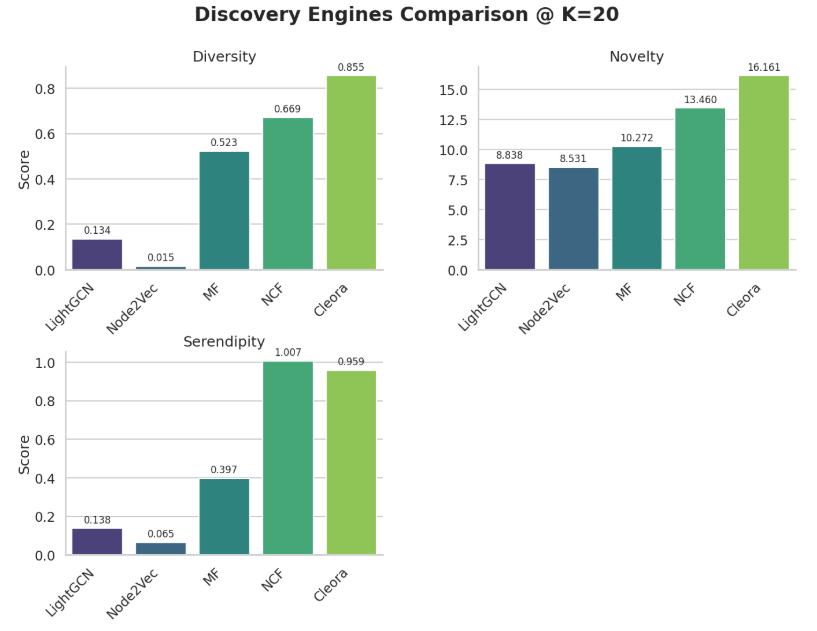
\includegraphics[width=0.9\linewidth]{discovery_metrics_comparison.png}
    \caption{Cleora and NCF significantly outperform accuracy-focused models in Novelty and Serendipity, highlighting their utility for exploration tasks.}
    \label{fig:discovery}
\end{figure}

\begin{itemize}
    \item \textbf{Novelty Leaders:} Cleora and NCF act as "Discovery Engines." Cleora achieves the highest Novelty score (\textbf{16.161}), recommending items with an average popularity of just ~28 interactions, whereas Node2Vec tends to recommend popular items (average popularity ~1150).
    \item \textbf{Diversity:} Cleora also leads in Diversity (\textbf{0.855}), followed by NCF (0.669). The accurate models, Node2Vec (0.015) and LightGCN (0.134), suffer from popularity bias, resulting in very low diversity scores.
    \item \textbf{Serendipity:} NCF achieved the highest Serendipity score (\textbf{1.007}), suggesting it is most effective at finding relevant items that are also surprising to the user.
\end{itemize}

\subsection{The Accuracy-Diversity Trade-off}
The experimental results highlight a clear distinction between "Safe" and "Discovery" engines:

\begin{figure}[H]
    \centering
    % Placeholder for the Accuracy vs Diversity scatter plot
    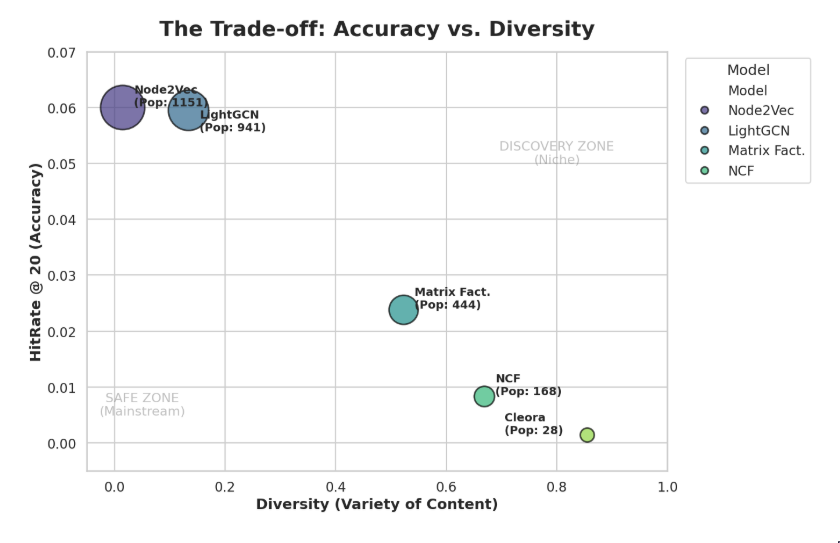
\includegraphics[width=0.8\linewidth]{accuracy_diversity_tradeoff.png}
    \caption{LightGCN and Node2Vec occupy the 'Safe Zone', while Cleora and NCF inhabit the 'Discovery Zone'.}
    \label{fig:tradeoff}
\end{figure}

\begin{itemize}
    \item \textbf{The Safe Zone:} Dominant in relevance but low in exploration. Ideal for primary feeds where trust is essential.
    \item \textbf{The Discovery Zone:} Excellent for surfacing the "long tail" of content but less reliable for immediate relevance.
\end{itemize}

\subsection{Final Recommendations}
Based on this analysis, we propose a hybrid deployment strategy:
\begin{enumerate}
    \item \textbf{Primary Feed:} Use \textbf{LightGCN} for high accuracy and user satisfaction.
    \item \textbf{Discovery Section:} Use \textbf{Matrix Factorization} or \textbf{NCF} to balance relevance with diversity ("Because You Watched").
    \item \textbf{Deep Dive:} Use \textbf{Cleora} to surface niche content that users rarely discover through popularity-biased models.
\end{enumerate}

\bibliographystyle{plain}
\begin{thebibliography}{9}

\bibitem{zhang2023inductive}
Canlin Zhang and Xiuwen Liu.
\newblock Inductive Link Prediction in Knowledge Graphs using Path-based Neural Networks.
\newblock \emph{arXiv preprint arXiv:2312.10293}, 2023.

\bibitem{teru2020inductive}
Komal K. Teru, Etienne Denis, and William L. Hamilton.
\newblock Inductive Relation Prediction by Subgraph Reasoning.
\newblock \emph{arXiv preprint arXiv:1911.06962}, 2020.

\bibitem{schlichtkrull2018modeling}
Michael Schlichtkrull, Thomas N. Kipf, Peter Bloem, Rianne van den Berg, Ivan Titov, and Max Welling.
\newblock Modeling Relational Data with Graph Convolutional Networks.
\newblock \emph{arXiv preprint arXiv:1703.06103}, 2017.

\end{thebibliography}

\appendix
\section{Appendix}

\begin{figure}[H]
    \centering
    % Placeholder for the system workflow diagram
    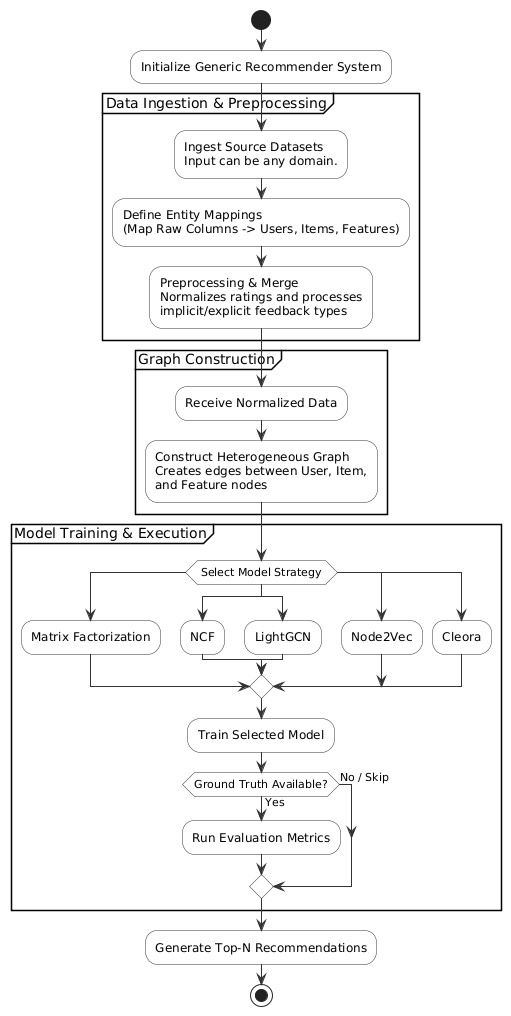
\includegraphics[width=1.0\linewidth, height=0.9\textheight, keepaspectratio]{workflow_diagram.png} 
    \caption{Generic Recommender System Workflow: From Data Ingestion to Recommendation Generation}
    \label{fig:workflow}
\end{figure}

\end{document}